\documentclass[sigplan,10pt,nonacm]{acmart}
\settopmatter{printfolios}

\makeatletter
\def\ps@headings{%
\def\@oddhead{\mbox{}\scriptsize\rightmark \hfil \thepage}%
\def\@evenhead{\scriptsize\thepage \hfil \leftmark\mbox{}}%
\def\@oddfoot{}%
\def\@evenfoot{}}
\makeatother
\raggedbottom
\graphicspath{ {./graphs/} }

\pagestyle{plain}
\settopmatter{printfolios=true}

%\usepackage[small,compact]{titlesec}
\usepackage{epsfig}
\usepackage{graphicx}
\usepackage{xspace}
\usepackage{listings}
\usepackage{multirow}
\usepackage{listings}
\usepackage{color}
\usepackage{caption}
\usepackage{subcaption}

\definecolor{mygreen}{rgb}{0,0.6,0}
\definecolor{mygray}{rgb}{0.5,0.5,0.5}
\definecolor{mymauve}{rgb}{0.58,0,0.82}

\lstset{ 
  backgroundcolor=\color{white},   % choose the background color; you must add \usepackage{color} or \usepackage{xcolor}; should come as last argument
  basicstyle=\footnotesize,        % the size of the fonts that are used for the code
  breakatwhitespace=false,         % sets if automatic breaks should only happen at whitespace
  breaklines=true,                 % sets automatic line breaking
  captionpos=b,                    % sets the caption-position to bottom
  commentstyle=\color{mygreen},    % comment style
  deletekeywords={...},            % if you want to delete keywords from the given language
  escapeinside={\%*}{*)},          % if you want to add LaTeX within your code
  extendedchars=true,              % lets you use non-ASCII characters; for 8-bits encodings only, does not work with UTF-8
  %firstnumber=1000,                % start line enumeration with line 1000
  frame=single,	                   % adds a frame around the code
  keepspaces=true,                 % keeps spaces in text, useful for keeping indentation of code (possibly needs columns=flexible)
  keywordstyle=\color{blue},       % keyword style
  language=C,                 % the language of the code
  morekeywords={*,...},            % if you want to add more keywords to the set
  numbers=none,                    % where to put the line-numbers; possible values are (none, left, right)
  numbersep=5pt,                   % how far the line-numbers are from the code
  numberstyle=\tiny\color{black}, % the style that is used for the line-numbers
  rulecolor=\color{black},         % if not set, the frame-color may be changed on line-breaks within not-black text (e.g. comments (green here))
  showspaces=false,                % show spaces everywhere adding particular underscores; it overrides 'showstringspaces'
  showstringspaces=false,          % underline spaces within strings only
  showtabs=false,                  % show tabs within strings adding particular underscores
  %stepnumber=2,                    % the step between two line-numbers. If it's 1, each line will be numbered
  stringstyle=\color{mymauve},     % string literal style
  tabsize=2,	                   % sets default tabsize to 2 spaces
  title=\lstname                   % show the filename of files included with \lstinputlisting; also try caption instead of title
}

\usepackage{url}
%\usepackage[hyphens]{url}
\usepackage{hyperref}
%\hypersetup{breaklinks=true}
%\usepackage[margin=10pt]{subcaption}
%\usepackage{subcaption}

% Other useful macros
\newcommand{\fixme}[1]{\textbf{FIX: #1}}
\newcommand{\codesm}[1]{\texttt{\small #1}}
\newcommand{\implication}{\vspace{0.1in} \noindent \emph{Implication:~}}
\newcommand{\fig}[4]{%
  \begin{figure}[ht]%
    %\frame{\includegraphics[#1]{#2}}
    \includegraphics[#1]{#2}
    \caption{{#3}}\label{#4}
\end{figure}
}

\newcommand{\question}[1]{\textbf{DOUBT: #1}}

\def \sec {\S}



\begin{document}
\widowpenalty=5000
\clubpenalty=5000


\title{\textsf{A Study on Query Optimization}}


\author{Anjali(anjali@wisc.edu) and Sakshi Bakshi(sbansal8@wisc.edu)}


\begin{abstract}
Query optimization is the part of the query process in which the database system compares different query strategies and chooses the one with the least expected cost. The query optimizer, which carries out this function, is a key part of the relational database and determines the most efficient way to access data. It makes it possible for the user to request the data without specifying how these data should be retrieved.

The cost of accessing a query is a weighted combination of the I/O and processing costs. The I/O cost is the cost of accessing index and data pages from disk. Processing cost is estimated by assigning an instruction count to each step in computing the result of the query.

In this project, we study the optimization done by PostgreSQL and SQLite by running the queries present in the SSB and TPC-H benchmarks. The results obtained help us to further investigate the query optimization techniques implemented by the two database systems.
\end{abstract}


\maketitle



\section{Introduction}
\label{sec:intro}

\fig{width=\columnwidth}{query}{\textmd{Stages of Query processing}}{fig:query}

Query optimization is part query processing in many relational database management systems. It determines the most efficient way to execute a particular query by evaluating the various query plans for it. Once the query is submitted to the database server, it is then passed to the parser and then passed to the query optimizer as shown in Figure~\ref{fig:query}.

There are many ways to implement a particular query depending on the schema and the complexity of the query. Different databases use different query optimizer which might result in different execution time for the same query when executed on different platforms. The fundamental task of a query optimizer is to select an algorithm from among the many available options that provides the answer with a minimum of disk I/O and CPU time.

Query optimizer~\cite{ref:sqlite3} frees the programmer from the task of selecting a particular query plan and allows the programmer to focus on high-level application issues. For simple query the choice of plan is mostly obvious but as schema and queries become important, the optimizer plays an inmportant role in simplifying the work of application development for the programmer.

The rest of the paper is organised as follows: Section~\ref{sec:db} gives an overview of the architecture for PostgreSQL and SQLite, Section~\ref{sec:bench} defines the benchmarks in detail, in Section~\ref{sec:results} we discuss the results. Finally, we discuss future work and conclude in Section~\ref{sec:future} and Section~\ref{sec:conclusion} respectively. 



\section{Databases}
\label{sec:db}

\subsection{PostgreSQL}
\fig{width=\columnwidth}{postgres}{\textmd{PostgreSQL Architecture}}{fig:postgres}

PostgreSQL~\cite{ref:pg1} is a relational database management system following a client-server architecture. At the server side an instance is created comprising of PostgreSQL's processes and shared memory which handles the access to the data. Client programs connect to the instance sending read and write operations. The overview of the architecture is shown in Figure~\ref{fig:postgres}.

An instance consists of multiple processes,  postmaster process, multiple postgres processes (one for each connection), WAL writer process, background writer process, checkpointer process and other optional processes like autovacuum launcher process, logger process , archiver process, stats collector process, WAL sender process (when streaming replication is active), WAL receiver process (when streaming replication is active) and background worker processes (in case a query gets parallelized). The client program sends the request to the instance. The instance itself does not directly write to disk instead it buffers the requested data in shared buffer. The flushing to disk is done at a later stage.

\subsection{SQLite}

\fig{width=\columnwidth}{sqlite}{\textmd{SQLite Architecture}}{fig:sqlite}

SQLite~\cite{ref:sqlite2} is an embedded file based relational database management system which can be linked statically or dynamically with the application program. It does not have a client-server database engine which makes the SQLite applications require less configuration. SQLite is called zero-conf as it does not require service management or access control based on password and GRANT.


SQLite complies with ACID  (atomicity, consistency, isolation, durability) properties and implements the SQL standard. It stores the entire database as a single disk file and all reads and write takes place directly on this file. 

SQLite database architecture is divided into two different sections called core and backend. Core contains Interface, Tokenizer, Parser, Code generator, and the virtual machine, which create an execution order for database transactions. Backend contains B-tree, Pager and OS interface to access the file system. Tokenizer, Parser and code generator is together named as the compiler which generates a set of opcodes that runs on a virtual machine.

\section{Benchmarks}
\label{sec:bench}

\subsection{TPC-H}
\fig{width=\columnwidth}{tpch}{\textmd{TPC-H schema}}{fig:tpch}

TPC-H~\cite{ref:tpch} is a decision support benchmark that consists of a suite of business oriented ad-hoc queries and concurrent data modifications. The queries and the data populating the database have been chosen to have broad industry-wide relevance while maintaining a sufficient degree of ease of implementation. It  evaluates the performance of various decision support systems by the execution of sets of queries against a standard database under controlled conditions.

The purpose of this benchmark is to reduce the diversity of operations found in an information analysis application, also retaining the application's essential performance characteristics, i.e, the level of system utilization and the complexity  of  operations.  A  large  number  of  queries  of  various  types  and  complexities  need  to  be  executed  to completely  manage  a  business  analysis  environment.

The  components  of  the  TPC-H  database  consists  of  eight  separate  and  individual  tables known as the Base Tables. The relationships between these tables are illustrated in Figure~\ref{fig:tpch}.




\subsection{SSB}
\fig{width=\columnwidth}{ssb}{\textmd{SSB schema}}{fig:ssb}

The Star Schema Benchmark (SSB)~\cite{ref:paper1} is designed to test star schema optimization to address the issues of TPC-H along with measuring performance of database  products  and test  a  new  materialization  strategy. The  SSB  is  a  simple  benchmark  that  consists  of  four  query flights,  four  dimensions,  and  a  simple  roll-up  hierarchy . The SSB is largely based on the TPC-H benchmark with improvements  implememting  a  traditional  pure  star-schema and allowing column and table compression.

The  SSB  is  designed  to  measure the performance  of  database products  against  a  traditional  data  warehouse  scheme.  It  implements  the  same  logical  data  in  a  traditional  star  schema whereas TPC-H models the data in pseudo 3NF schema.

Modifications to  the  TPC-H  schema were made to transform  it  into  a star  schema  form.  The TPC-H tables LINEITEM and ORDERS are combined into one sales fact table named LINEORDER. The PARTSUPP table  is  dropped.  The comment  attributes  for LINEITEMS, ORDERS,  and  shipping instructions  are  also  dropped. A  dimension  table  called DATE is  added  to  the  schema as  is  in  line  with  a  typical  data  warehouse. LINEORDER serves  as the fact  table.  Dimension Tables  are  created  for CUSTOMER, PART, SUPPLIER and DATE.

SSB concentrates on queries that select from the LINEORDER table  exactly  once.  It  avoids   the use  of  self-joins  or  subqueries  as  well  as  or  table  queries also  involving LINEORDER.  The  classic  warehouse  query selects  from  the  table  with  restrictions  on  the  dimension table attributes. SSB supports queries that appear in TPC-H. SSB consists of one large fact table (LINEORDER) and four dimensions tables (CUSTOMER, SUPPLIER, PART and DATE).

\section{Results}
\label{sec:results}

\subsection{Method}
We run all our experiments on Cloudlab [5] xl170 machine, with a ten-core Intel E5-2640v4 running at 2.4 GHz, 64GB ECC Memory (4x 16 GB DDR4-2400 DIMMs), Intel DC S3520 480 GB 6G SATA SSD and 10Gbps NIC. We run on Ubuntu 18.04 (4.15.0-55-generic). We performed all the experiments on PostgreSQL version 10.10 and SQLite3 version 3.22.0. The buffer pool for each system is set to 2MB.. PostgreSQL is configured to run with zero parallelism to get a baseline comparison between the two systems since SQLite runs in a single thread. We also make sure that each query runs on a single core. To achieve zero paralleism following configurations are set in PostgreSQL:

\texttt{max\_worker\_processes:} Maximum number of background processes that the system can support.
We have set this parameter to 1.

\texttt{max\_parallel\_workers\_per\_gather:} Maximum number of workers that can be started by a single Gather or Gather Merge node. Gather node has one child plan which requires some number of background workers to execute the rest of the portion in parallel. We set this parameter to 0.

We first measure the execution times for both the benchmarks and then compare the query plans generated for few queries from TPCH to understand the difference in execution time.
We compare results of TPC-H benchmark on PostgreSQL from previous setting with results obtained by turning parallelism on. In the new setting, \texttt{max\_worker\_processes} is set to 30 and \texttt{max\_parallel\_workers\_per\_gather} is set to 20.

\subsection{Execution Time}
\label{sec:time}

\fig{width=\columnwidth}{tpch_result}{\textmd{TPC-H result}}{fig:tpch_result}
\fig{width=\columnwidth}{ssb_result}{\textmd{SSB result}}{fig:ssb_result}
\fig{width=\columnwidth}{TPC-H_Postgres_Parallel_vs_Non-Parallel_Query_Execution}{\textmd{TPC-H result}}{fig:tpch_pg_parallel_non_parallel}

The total execution time for TPCH is shown in Figure~\ref{fig:tpch_result}. We observe that even though PostgreSQL is a much more complex system than the light-weight SQLite, it is not always faster. SQLite is competitive in some cases. The same behaviour is observed for SSB in Figure~\ref{fig:ssb_result}. These results give us an overall picture of the execution time of one system in comparison with the other.

Figure \ref{fig:tpch_pg_parallel_non_parallel} compares the results of PostgreSQL with  {max\_parallel\_workers\_per\_gather} set to 0 versus {max\_parallel\_workers\_per\_gather} = 20. The results show that the run times of almost all the queries decrease significantly upon changing this parameter. It was noted that the queries for which run times didn't change (Q2, Q13, Q18, Q21) were the ones that didn't use Gather node in their plans at all. <This further strengthens our asssumption that parallelism affect postgres queries significantly and this parameter should be set to 0 for analysis with sqlite? >



\subsection{Query Plan Comparison}
\label{sec:plan}

\subsubsection{Almost same time}
\fig{width=\columnwidth}{tpch-postgres-16}{\textmd{PostgreSQL plan for query 16}}{fig:tpch-postgres-16}

\begin{figure*}[ht]
\centering
     \begin{subfigure}[b]{0.4\textwidth}
         \centering
         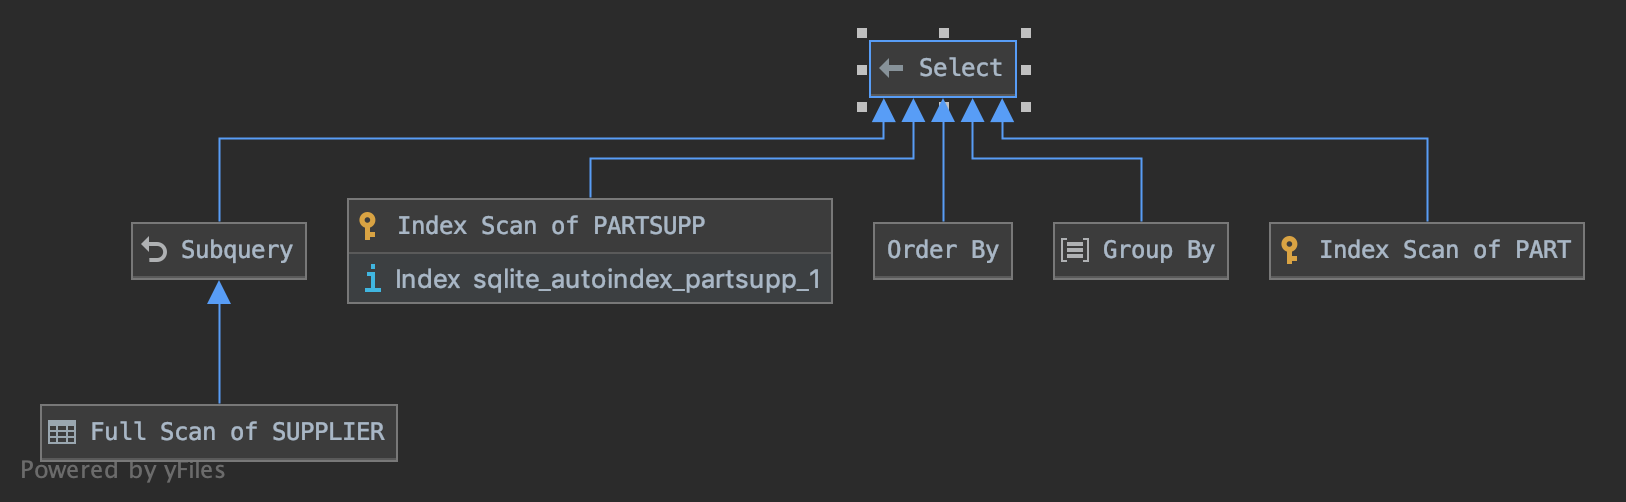
\includegraphics[width=\columnwidth]{tpch-sqllite-16}
         \caption{SQLite query plan 16 steps}
         \label{fig:tpch-sqllite-16}
     \end{subfigure}
     \hfill
     \begin{subfigure}[b]{0.4\textwidth}
         \centering
         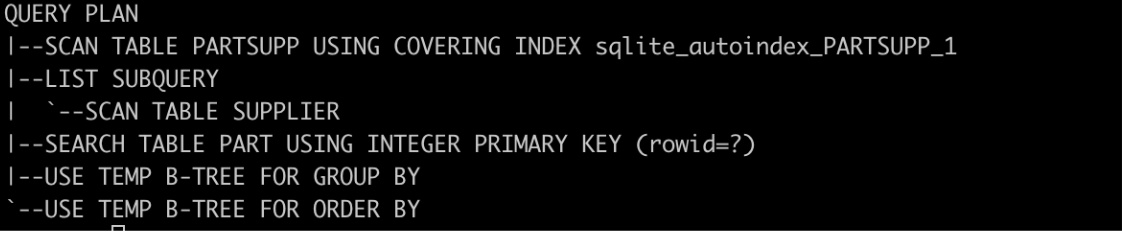
\includegraphics[width=\columnwidth]{sqlite-16-2}
         \caption{SQLite query plan 16}
         \label{fig:sqlite-16-2}
     \end{subfigure}

        \caption{SQLite plan for query 16}
        \label{fig:sqlite-16}
\end{figure*}

We now look at query 16 represented in Listing~\ref{q16} from the TPCH benchmark suite. In this query is the Parts/Supplier Relationship Query that returns how many suppliers can supply parts with given attributes. This query has almost same time for both, PostgreSQL and SQLite.

Figure~\ref{fig:tpch-postgres-16} shows the query plan generated for this query in PostgreSQL, we observe that it does a full scan of all the tables followed by some hash joins, sort, aggregate and then sort again. If we look at the query plan for SQLite in Figure~\ref{fig:sqlite-16}, we observe that it also does a scan of all the tables and execute a similar query plan. Since the query plans generated by both are significantly similar and this query does not contain the big table, LINEITEM, therefore the scans take similar time even though SQLite does an index scan. All this add up to almost same time for this particular query in both the databases.\\

\begin{minipage}{\linewidth}
\begin{lstlisting}[breaklines=true, numbers=none, label=q16, caption=Query 16]
select p_brand, p_type, p_size, count(distinct ps_suppkey) as supplier_cnt
from
partsupp, part
where
p_partkey = ps_partkey
and p_brand <> '[BRAND]'
and p_type not like '[TYPE]%'
and p_size in ([SIZE1], [SIZE2], [SIZE3], [SIZE4], [SIZE5], [SIZE6], [SIZE7], [SIZE8])
and ps_suppkey not in (
select s_suppkey
from supplier
where
s_comment like '%Customer%Complaints%'
)
group by p_brand, p_type, p_size
order by
supplier_cnt desc,
p_brand,
p_type,
p_size;;
\end{lstlisting}
\end{minipage}



%\fig{width=\columnwidth}{tpch-sqllite-16}{\textmd{TPCH result}}{fig:tpch-sqllite-16}



\subsubsection{PostgreSQL faster}
\fig{width=\columnwidth}{tpch-postgres-9}{\textmd{PostgreSQL plan for query 9}}{fig:tpch-postgres-9}

\begin{figure*}[ht]
\centering
     \begin{subfigure}[b]{0.4\textwidth}
         \centering
         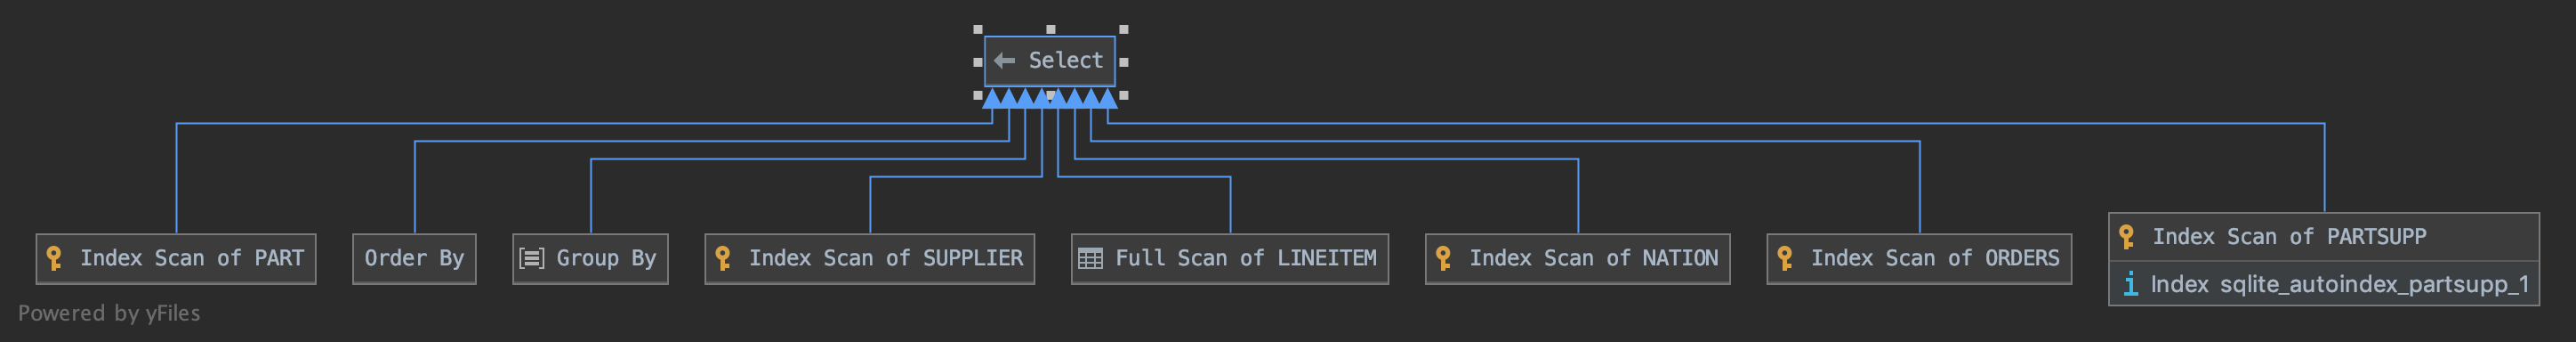
\includegraphics[width=\columnwidth]{tpch-sqllite-9}
         \caption{SQLite query plan 9 steps}
         \label{fig:tpch-sqllite-9}
     \end{subfigure}
     \hfill
     \begin{subfigure}[b]{0.4\textwidth}
         \centering
         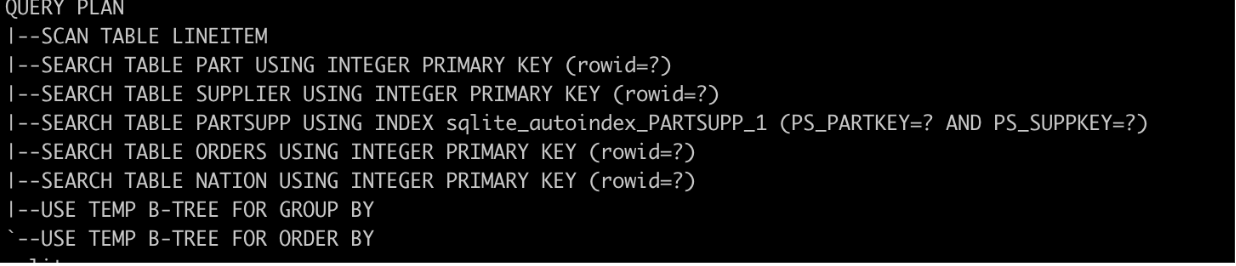
\includegraphics[width=\columnwidth]{sqlite-9-2}
         \caption{SQLite query plan 9}
         \label{fig:sqlite-9-2}
     \end{subfigure}

        \caption{SQLite plan for query 9}
        \label{fig:sqlite-9}
\end{figure*}
%\fig{width=\columnwidth}{tpch-sqllite-9}{\textmd{TPCH result}}{fig:tpch-sqllite-9}
Query 9 shown in Listing~\ref{q9} called Product Type Profit Measure Query which determines how much profit is made on a given line of parts, broken out by supplier nation and year. This query takes longer execution time SQLite.

Figure~\ref{fig:tpch-postgres-9} shows the query plan for PostgreSQL where we observe that it does full scan of all the tables followed by hash join and aggregate at the end. In SQLite shown in Figure~\ref{fig:sqlite-9}, we see many index scans. We also see that this query has LINEITEM which is a big table and hence, selectivity for this particular query is very high. Therefore, index scan in this scan becomes expensive over full scan which is seen by the lower execution time for PostgreSQL.

\begin{minipage}{\linewidth}
\begin{lstlisting}[breaklines=true, numbers=none, label=q9, caption=Query 9]
select nation, o_year, sum(amount) as sum_profit
from (
select
n_name as nation,
extract(year from o_orderdate) as o_year,
l_extendedprice * (1 - l_discount) - ps_supplycost * l_quantity as amount
from part, supplier, lineitem, partsupp, orders, nation
where
s_suppkey = l_suppkey
and ps_suppkey = l_suppkey
and ps_partkey = l_partkey
and p_partkey = l_partkey
and o_orderkey = l_orderkey
and s_nationkey = n_nationkey
and p_name like '%[COLOR]%'
) as profit
group by
nation,
o_year
order by
nation,
o_year desc;
\end{lstlisting}
\end{minipage}

\subsubsection{SQLite faster}

\fig{width=\columnwidth}{tpch-postgres-4}{\textmd{PostgreSQL plan for query 4}}{fig:pgsql-4}

\begin{figure*}[ht]
\centering
     \begin{subfigure}[b]{0.4\textwidth}
         \centering
         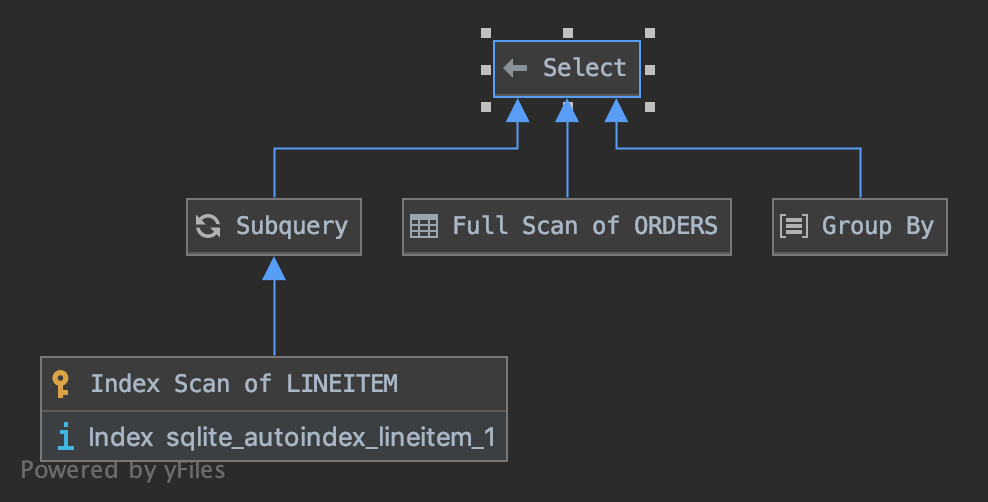
\includegraphics[width=\columnwidth]{tpch-sqllite-4}
         \caption{SQLite query plan 4 steps}
         \label{fig:tpch-sqllite-4}
     \end{subfigure}
     \hfill
     \begin{subfigure}[b]{0.4\textwidth}
         \centering
         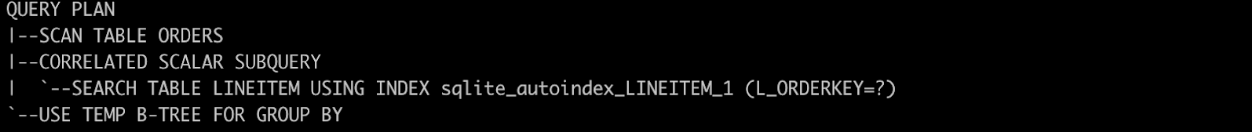
\includegraphics[width=\columnwidth]{sqlite-4-2}
         \caption{SQLite query plan 4}
         \label{fig:sqlite-4-2}
     \end{subfigure}

        \caption{SQLite plan for query 4}
        \label{fig:sqlite-4}
\end{figure*}
%\fig{width=\columnwidth}{tpch-sqllite-4}{\textmd{TPCH result}}{fig:tpch-sqllite-4}
Query 4 shown in Listing~\ref{q4} is called Order Priority Checking Query which finds how well the order priority system is working and gives an assessment of customer satisfaction. This query runs faster in SQLite.

The query plan for PostgreSQL is shown in Figure~\ref{fig:pgsql-4} and SQLite is shown in Figure~\ref{fig:sqlite-4}. This query has an inner query which is called a correlated subquery~\cite{ref:sqlite1} which depends on the outer query. The selectivity of this query is around 3\%. In case of PostgreSQL we observe that it does a full scan of all the tables whereas SQLite uses an index scan. In queries where selectivity is low, index scan is faster, therefore, we see that SQLite performs better than PostgreSQL. Since the table in question is Lineitem table which occupies 750 MB on disk out of 1GB of the entire TPC-H database, the effects seem more significant in this query than the others.

\begin{minipage}{\linewidth}
\begin{lstlisting}[breaklines=true, numbers=none, label=q4, caption=Query 4]
select o_orderpriority, count(*) as order_count
from
orders
where
o_orderdate >= date '[DATE]'
and o_orderdate < date '[DATE]' + interval '3' month
and exists (
select * from lineitem
where l_orderkey = o_orderkey and l_commitdate < l_receiptdate
)
group by o_orderpriority, order by, o_orderpriority;
\end{lstlisting}
\end{minipage}







\section{Future Work}
\label{sec:future}
In this project we looked at two benchmarks. It can be extended to more benchmarks which are more closely suited for application where SQLite is used over PostgreSQL. The project can also extended to create a standalone service that takes SQLite queries and outputs a generic optimised physical plan in a DAG form for other services like Hustle to ingest and execute. 

Also, the query plan generated by SQLite is not as thorough and detailed as PostgreSQL, so it was very difficult to make concrete conclusions in some cases. One can also think about implementing this part so that SQLite output better and more detailed logical plan that helps in further analysis.

\section{Conclusions}
\label{sec:conclusion}
In the preceding sections we compared the performance of SQLite and PostgreSQL on two benchmarks, TPC-H and SSB. We observed that SQLite was slow in most of the cases but it did perform almost as same and even better in some cases. We can attribute this performance difference between the two databases to the difference in the architecture and the use-case for each in different scenarios.

PostgreSQL follows the client/server architecture whereas SQLite is file based (embedded). Although PostgreSQL has more complex architecture but it performs efficiently in most cases. Also, the benchmarks we used TPC-H and SSB are for decision support for business and data warehouse respectively which are more suited to the use-case for PostgreSQL, which also explains its better performance in these benchmarks. SQLite~\cite{ref:compare} is light-weight and suited for applications like IoT, embedded devices, low-medium traffic websites, etc. 

When we look at the difference in their query plans we can see that the index scan that is used by SQLite in most cases becomes expensive as the selectivity increases. Also, the current implementation of SQLite uses only loop joins, i.e, joins are implemented as nested loops which also add to this overhead most of the time.

PostgreSQL does a sequential full scans followed by hash-joins in most cases. In comparision to nested loop joins, hash-joins are better which is evident from the better performance of PostgreSQL in most cases. It only performs worse in cases where the selectivity is low.
 





{
\bibliographystyle{abbrv}
\bibliography{paper}
}
\end{document}
